
\documentclass[oneside,a4paper,titlepage]{article}
\usepackage{blindtext}
\usepackage[utf8]{inputenc}
\usepackage{verbatim} 
\usepackage{graphicx}
\usepackage{color}
\usepackage{float}
% hidelinks fjerner farvede kanter omkring links og refferencer
\usepackage[hidelinks]{hyperref}
\usepackage{lipsum}

% Mappe hvori billeder ligger
\graphicspath{ {graphics/} }

% Tekst som står først i figur captions "{Figure/Figur} 3: Pixelering der fremkommer..."
\renewcommand{\figurename}{Figur}


% supresses errors during compilation
% \batchmode

\title{Ray Tracing}
\author{P1 B2-28}
\date{\today}

\begin{document}
\maketitle

\renewcommand{\abstractname}{Abstrakt}
\begin{abstract}
Abstract text placeholder, lorem ipsum dolor sit amet...
\end{abstract}

\tableofcontents
\clearpage

% sections
Selvom vi ikke tænker på det så ofte, så er lamper en stor del af vores hverdag. De står i vores hjem, på vores gader, på vores arbejdsplads - ja de er stort set overalt. Men hvorfor er lamper egentlig så udbredte? Det er de, fordi lamper bliver brugt til at skabe lys. Belysning kan bidrage til mange ting som at læse, arbejde mere koncentret eller til at skabe hygge og stemning i et rum, der ellers ville have været koldt og kedeligt. 
\newline Lamper findes i mange forskellige typer og mange forskellige steder. Der er læselamper, arbejdslamper, loftlamper, udendørslamper osv. og de tjener allesammen forskellige formål, men fælles for dem er, at de skaber lys steder hvor der ellers ikke ville have været lys. 
I dag findes der utroligt mange forskellige lampedesigns, og de er ikke allesammen lige gode. Dette vil sige at nogle lamper har meget dårlig belysning. Dette er et problem, da undersøgelser har vist at dårlig belysning kan føre til blandt andet øjenskader, hovedpine samt ondt i nakke og hals \cite{lys_konsekvenser}. Andre problemer kan også opstå, hvis en lampe har en for kraftig belysning, og derfor er blændende eller hvis f.eks en udendørs lampe ikke lyser tilstrækkeligt, og man derfor vælter, fordi man ikke kan se noget. 
Så selvom lamper spiller en stor rolle i vores hverdag, så er det vigtigt at kunne visualisere hvordan lys udbreder sig fra en lampe, så man kan undgå dårlig belysning. 
\newline Man kan derfor argumentere for at det essentielle ved en lampe ikke er dens design, men er det lys som den udsender, herunder mønster og farve, samt lysets indflydelse på indretning og belysning. Med afsæt i denne argumentation har vi derfor valgt at arbejde med visualisering af lyset fra lamper.

\subsection{Motivation}

Som studerende på software synes vi, at det kunne være interresant at arbejde med et håndterbart problem som der ville kunne findes en teknologisk løsning på. 
\newline Gruppens mål er derfor at finde et relevant problem indenfor visualisering af lyset fra lamper, og derudfra lave en teknologisk løsning på problemet. Som gruppe er vi motiveret af, at vi kan designe og implementere software med henblik på at finde en god løsning på et relevant problem. 

\subsection{Initierende problem}

I indledningen slog vi som gruppe fast, at vi gerne ville arbejde med visualisering af lyset fra lamper. På baggrund af vores viden om lys fra lamper, samt de erfaringer og diskussioner vi har foretaget os som gruppe, har vi valgt at opstille følgende initierende problem:

Forbrugeren kan ikke visualisere, hvordan lyset udbreder sig fra en lampe uden at købe og installere lampen.

\section{Problemanalyse}
\subsection{Begrebsligørelse}
Der er indtil videre blevet  argumenteret for relevansen af det initierende problem, og det er i den sammenhæng derfor nødvendigt at redegøre for nogle vigtige emner og ord indenfor problemfeltet. 

Formålet med dette afsnit er at beskrive vigtige begreber samt kort at give en beskrivelse af, hvordan de forskellige ord og begreber skal forstås i den videre rapport. Begreberne som fremgår i følgende afsnit danner grundlag for forståelsen af det initierende problem. Disse begreber er følgende: Forbruger, visualisering, lys og lamper.

% \subsubsection{Køber}
% En køber er en person, der køber et produkt eller tjenesteydelser \cite{ddo_forbruger}.  Køberen står altså i denne sammenhæng i modsætning til producenterne.
% I denne rapport opfattes køberen som den person der køber lampen. Det vil altså sige, at der i dette tilfælde ikke nødvendigvis er tale om personer der til dagligt bruger eller bliver påvirket af lampen.

\subsubsection{Forbruger}
En forbruger er en privatperson som køber et produkt eller tjenesteydelser. “Forbruge” betyder at “bruge noget”, og en forbruger køber derfor produkter med henblik på at tilfredsstille nogle behov \cite{forbrugerportalen}. En bevidst forbruger, vil derfor ofte lede efter produkter der opfylder deres behov. Man antages også for at være forbruger af en varer hvis man til daglig benytter sig af eller bliver påvirket af en given lampe. 

I vores rapport udvider vi definitionen af forbruger til, at en forbruger også kan være en erhvervsperson der køber en lampe til brug i virksomheden. Derudover hører en kunde også til under begrebet forbruger, da det er kunderne som køber lamperne. 

%\subsubsection{Sælger}
%En sælger er den person eller virksomhed der sælger et produkt eller %tjenesteydelser. I rapporten opfattes sælgeren som værende en person %eller virksomhed, der sælger lamper til forbrugeren. 

\subsubsection{Visualisering}
At visualisere, betyder at skabe et billede på baggrund af noget \cite{ddo_visualisering}. Dette kan til dels være tanker, som omsættes til billeder for det indre øje. Det kan også være en række data, som omsættes til billeder, så de er nemmere at forstå.
Visualisering kan være et redskab til at skabe en forståelse for det der visualiseres. Dette kan f.eks være prototyper af lamper, der kan give en forståelse for hvordan lyset udbreder sig fra en lampe. Derudover er der inden for computergrafik metoder til at skabe billeder på baggrund af 3D-modeller, så man f.eks. kan lave et delvist realistisk billede af en lampe, og på den måde få en forståelse for hvordan lampen ser ud i virkeligheden og hvordan dens lys udbredes. Forskellige teknologier til visualisering er uddybet senere i rapporten under afsnit \ref{sec:teknologianalyse}. 

\subsubsection{Lys}
Der er forskellige opfattelser af hvad lys det indebærer. Hvis vi tager udgangspunkt i Karsten Rottwitt, som er professor ved DTU fotonik, så påstår han at lys er:

“Lys er andet end synligt lys. For mig er lys et elektromagnetisk felt, som har en høj frekvens”
- Karsten Rottwitt\cite{def_lys}.

Han mener også, at der er en hårdfin grænse for hvornår lys kan betegnes som lys, denne grænse er dog først i spil når vi snakker om UV-lys og infrarødt lys \cite{def_lys}. 
Andre er ikke enige med Karsten Rottwitt om hvordan definitionen af lys er. Tager vi nu udgangspunkt i Britannica \cite{britannica_lys}, så betegnes lys, som magnetiske stråler, som det menneskelige øje kan opfange - Hvilket vil sige, lys med en bølgelængde mellem 380 og 750 nanometer, også kaldet synligt lys. 

Det er denne definition, som rapporten vil tage udgangspunkt i. Dette er valgt, da det er oplagt at kombinere synligt lys og lamper \cite{def_lys}.

Det lys som kommer fra en lampe, er selvfølgelig af forskellig kvalitet. Kvalitet kan ligesom lys, betegnes på mange måder, herunder kan vi snakke om hvorvidt en lyskilde er af god kvalitet, hvis den er energivenlig eller om det kun kommer an på hvor gode de er til at eftergive farvet lys. 
Afhængigt af hvor man skal bruge lyset, kan nogle former for lys være bedre egnet end andre. Her menes der om hvorvidt lyset skal være varmt eller koldt. Integral-led er et firma med over 25 års erfaring\cite{integral_led}, og har opstillet nogle foretrukne steder at bruge de forskellige typer af lys:

Varm / varm hvid = Stue, soveværelse eller gange.
Hvid / kold hvid = Køkken, studie, badeværelser, skrivebord, kontor eller butikker\cite{varm_kold}.

Ud fra disse foretrukne placeringer, opstillet af integral-led, kan vi antage at lys kvaliteten blandt andet afhænger af hvor lyset skal bruges. Hvis det er i et stille og roligt miljø, med henblik på at slappe af, er det måske at foretrække det varme lys, hvormid de steder hvor det er nødvendigt at have skarpt lys, for evt. at kunne se detaljer eller koncentrere sig, er det kolde lys at foretrække.

\subsubsection{Pærer}
I denne rapport forstås en pærer, som en enhed der ved hjælp af elektricitet udsender lys. Herunder er der forskellige typer pærer, men hvilken skal man vælge? Sparepærer, LED eller halogen?
Da der findes så mange pærer, er der visse ting, der er værd at overveje. En pærer har en Ra-værdi, som bruges til at bedømme hvor god en farvegengivelse pæren har. Ra-skalaen går helt op til 100, hvor det kun er sollys som har en Ra-værdi på 100, der er dog nogle typer af pærer, som næsten kan ramme de 100 Ra.\cite{halogen_paere}

En anden overvejelse er hvor energivenlig pæren skal være, da det svinger meget afhængigt af hvilken pærer der bruges. Ser man på nogle af fordelene ved LED pærer, så er de billige i drift da de har en lang levetid, på ca. 25 år, samt et lavt energiforbrug\cite{LED}, 4-5 gange så lidt, i forhold til halogenpæren, som kun har en levetid på ca. 2år\cite{vaelg_paere}. 
Der findes pærer, som eftergiver bedre end andre, og blandt toppen findes Halogen pæren, som kan komme op på 99 Ra, hvilket næsten giver perfekt lys\cite{halogen_paere}. 

Fælles for alle typer af pærer, kan kvaliteten svinge afhængig af hvilken producent. Men hvilken pærer der er bedst, er svært at sige. De har alle sine fordele og ulemper, men går man efter levetid er LED pæren bedst, samt der er mange penge at spare i løbet af de år. Halogen pæren er rigtig god til at eftergive farve, da den har en kelvin på ca. 2500-3000, samt en høj Ra-værdi. Er det en god grundbelysning, samt rimelig billig i indkøb samt drift, så er sparepæren en god løsning, undtagen hvis det er til udendørs brug, da pæren mister lys og levetid ved -20 grader\cite{sparepaerer}.

Det kan konkluderes udfra ovenstående, at kvaliteten af en lyskilde, afhænger af hvor lyset skal bruges, for de forskellige pærer er alle gode, afhængigt af hvor den placeres. Udover kvaliteten af pæren, kan det antages at de forskellige pærer afgiver lys på forskellige måder og dermed kan det være svært at forudse hvordan lampen og lyset kommer til at se ud.  


\subsubsection{Lamper}
Formålet med dette afsnit er at afgrænse definitionen af hvad en lampe er i vores kontekst og hvordan begrebet skal forstås i rapporten.
Der findes mange forskellige definitioner på hvad en lampe faktisk er, og det viser sig ifølge American Heritage® Dictionary of the English Language \cite{american_heritage}, at begrebet ’lampe’ faktisk dækker over mange forskellige ting. 

American Heritage definerer en lampe som værende én eller flere af følgende:

En af flere forskellige enheder, der genererer lys og ofte varme, især:
\begin{enumerate}
    \item En elektrisk anordning, der har en sokkel til en pære, især et fritstående stykke møbel.
    \item En anordning, der afgiver ultravoilet, infrarød, eller anden stråling, som kan anvendes til terapeutiske formål.
    \item En pære: en projektør/et spot(light), udstyret med metalhalogenlampe.
    \item En lanterne eller armatur, der afgiver lys ved afbrænding af gas, ofte ved brug af en kappe.
\end{enumerate}

Idet der er så mange forskellige definitioner på en lampe, er vi, i konteksten af vores projekt, nødsaget til at afgrænse begrebet til noget mere specifikt. Da vi vil hjælpe forbrugeren, med at visualisere lampen i et givet rum, tager vi udgangspunkt i en mere normal lampe. Hvis man kigger på de tidligere definitioner af en lampe, kan man forestille sig utroligt mange apparaturer, som kan kaldes for en lampe. Lige fra ultraviolette lamper, der bruges i natklubber med fluoserende formål, til infrarøde lamper, der kan bruges i medicinske/terapeutiske sammenhænge, fx til at løsne og afspænde musklerne \cite{lys_terapi}. Der findes også lamper, der afgiver lys og varme ved afbrænding af fx gas, såsom en lanterne. For at afgrænse alle disse definitioner, vil en lampe i det videre arbejde med rapporten opfattes som en indendørs anordning, hvori der kan isættes en pære, som kan udsende lys, der evt. afskærmes af anordningen.

\paragraph{Opsummering}
Ud fra de ovenstående afsnit i begrebsliggørelsen, kan der nu kortfattes at der senere i denne rapport anvendes de omtalte begreber med følgende betydning:
\begin{enumerate}
	\item Forbruger: En person der køber en lampe med henblik på brug i hjemmet eller i en virksomhed.
	%\item Sælger: En person eller virksomhed der sælger produkter.
	\item Visualisering: Skabelsen af et billede på baggrund af noget, der evt. ønskes lettere forståeligt.
	\item Lys: Den elektromagnetiske stråling der er synligt for øjet (Synligt lys).
	\item Pære: En enhed der ved hjælp af elektricitet udsender lys.
	\item Lampe: En indendørs anordning hvor der kan isættes en pære, som udsender lys der evt. afskærmes af anordningen.
\end{enumerate}
Ud fra de ovenstående begreber, skulle der nu være en entydig forståelse af det initierende problemet, som gør at problemet nu kan analyseres videre i de kommende afsnit.






\subsection{e-handel}
e-handel er elektronisk handel via internettet. På internettet kan sælgere inden for e-handel have såkaldte e-butikker, hvor kunder kan købe varer. E-butikker er ofte udformet således at kunden kan se billeder og informationer omkring sælgerens varer og derudfra kan kunden vælge at lægge varerne i en virtuel indkøbskurv, hvor kunden til sidst indtaster de nødvendige oplysninger for at købe og modtage varerne.
%http://ordnet.dk/ddo/ordbog?query=ebutik
%http://ordnet.dk/ddo/ordbog?query=ehandel


Blandt de mange forskellige varer, der sælges via e-butikker, er det her relevant at tale om e-handel med lamper. Nedenstående figur \ref{e_handel_med_lamper} illustrerer princippet bag en lampesælgers salg af lampe til en kunde via en e-butik.
\begin{figure}[H]
	\centering
	\def\svgwidth{\columnwidth}
	\input{./e_handel_med_lampe.pdf_tex}
	\caption{Princippet bag handel af en lampe via en e-butik.}\label{e_handel_med_lamper}
\end{figure}

På figur \ref{e_handel_med_lamper} er det vist hvordan e-handlen starter med at kunden får et udvalg af lamper fra e-butikken. Kunden sender så en bestilling, som via e-butikken sendes videre til lampesælgeren, og til sidst sendes lampen til kunden. Dog ender handlen ikke nødvendigvis her, da kunden kan sende lampen retur såfremt at gældende lovgivning og købsbetingelser muliggører dette. For at undersøge lovgivningen nærmere kan man tage udgangspunkt i den danske lov om forbrugeraftaler.
%https://www.retsinformation.dk/forms/r0710.aspx?id=160666#Kap4

I lovens kapitel 1, § 1, stk. 2, nr. 1, fremgår der at lovens bestemmelser for fortrydelsesret gælder for aftaler, som er indgået ved fjernsalg. For en  fjernsalgsaftale gælder der, at aftalen om varer, er indgået gennem fjernkommunikation, hvor den erhvervsdrivende og forbrugeren ikke mødes fysisk (jf. kap. 1, § 3, nr. 1).

Ser man nu på loven i forbindelse med e-handel, foregår fjernkommunikationen gennem internettet via e-butikken, hvor fjernsalgsaftalen udføres i form af brugerens bestilling af f.eks. en lampe. Dette gør at fortrydelsesretten gælder ved e-handel.

Fortrydelsesretten er en forbrugers mulighed for at melde sig ud af en aftale, herunder køb af lamper ved e-handel. Hvis en en forbruger eksempelvis køber en lampe via en e-butik, har forbrugeren mulighed for at fortryde købet inden 14 dage ved at meddele dette til den erhvervsdrievende (jf. kap. 4, § 19). Herefter har forbrugeren 14 dage til at returnere varen (jf. kap. 4, § 24). Hvis varens værdi er forringet som følge af forbrugeren unødvendige håndtering af varen for at inspicere denne, så hæfter forbrugeren for denne værdiforringelse (jf. kap. 4, § 24, stk. 5). Dvs. at hvis en bruger installerer og bruger lampen, hvor der f.eks. tilpasses ledninger, så kan lampens værdi forringes og forbrugeren skal hæfte for dette. 








\subsection{Teknologianalyse}

Vi ser en tydelig mulighed for at assistere forbrugere med at træffe et valg når det kommer til (køb af vare på nettet | bestemmelse af optimale lysforhold i hjemmet | visualisering af et tilkøbt element i forbrugernes dagligdag/hjem). Dette vil sandsynligvis kunne løses ved hjælp af bedre købsvejledning eller værktøjer til at assistere forbrugeren i en købssituation hvor en prøve ikke kan stilles til rådighed eller at returnere varen er umuligt eller for omfattende en process.

% // redegørelse
Blot at vælge en lampe fra et katalog er problematisk hvis der ikke er billeder af lampen som 
\begin{enumerate}
    \item Fremviser lampen som møbel, rent visuelt, det fysiske design og 
    \item Viser hvordan lys kastes af lampen. En god løsning vil være at have en fysisk model placeret i en kontekst hvor man kan komme og se lampen og se lyset i sammenspil med anden indretning, sålledes som f.eks. Ikea gør.
\end{enumerate}
\begin{figure}[H]
    \centering
    \fbox{\rule{\textwidth}{5cm}}
    \caption{Ikea hus billede}
    % https://www.pinterest.com/pin/6685099420243693/
\end{figure} 

Man vil også kunne skabe billige prototyper af lamper vha. 3D printer tekniker. Disse ville eventuelt være mulige at tage med hjem for at teste hvordan en lampe passer ind i det rum den egentligt er købt til, men fordi plastik vejer mindre end metal, glas og andre tunge materialer som lamper kan være produceret af, kunne man forestille sig ophængs metoder der ikke nødvendiggør at bore huller i væge før man har set om lampen passer ind i rummet.
En tredje metode kunne være at konstruere en 3D model af lampen og køre en simulation af hvordan den kaster lys, dette koncept vil også kunne udvides til at en forbruger kan modellere deres eget hjem og placere lampen i den model, eller det kan anvendes af sælgere som et værktøj til at vejlede forbrugeren til at gøre det rigtige køb.

% Indledning over

\subsubsection{Teknologier til visualisering}
For at undersøge hvilke teknologier der kan anvendes til visualisering, er der i dette afsnit en række teknologier og metoder, som alle er relevante i forhold til at visualisere en lampe. Formålet med afsnittet er at få en forståelse af hvilke teknologier der allerede eksisterer inden for visualisering, og finde ud af hvilke metoder der er bedst i forhold til visualisering af lamper for forbrugere der handler via internettet.

\paragraph{3D print}
En teknologi som sælgeren vil kunne være i stand til at bruge er 3D printere. De fleste 3D printere kan typisk benytte to slags plastik: Acrylnitrol Butadien Styren (ABS) \cite{hvordan_3Dprinter} og Poly Lactic Acid (PLA) \cite{hvordan_3Dprinter}, plasten kommer som en lang tråd på en rulle, som bliver sat på siden af printeren. Plasttråden bliver herefter ført gennem et rør ned til 3D printerens hoved, lige før plasten kommer ud af hovedet bliver det varmet op til knap 200 grader \cite{hvordan_3Dprinter}. Den flydende plastik bliver nu lagt i tynde lag typisk op 0.1mm størrelse, derfor størkner plasten hurtigt og smelter sig sammen med det underliggende lag, det at printe et lag af gangen er en additiv produktionsmetode \cite{additiv_produktion}. Sælgeren vil kunne bruge denne teknologi til at lave en demostrations vare som forbrugeren kunne tage med hjem, men da vi fokuserer på sælgere inden for e-handel vil dette ikke være en mulighed da e-handel som sagt ikke er en fysisk butik. I stedet kan sælgeren give forbrugeren en fil, så forbrugeren selv vil være i stand til at lave en 3D print af en bestemt lampe, dette vil dog kræve at forbrugeren har en 3D printer og masser af tid da store objekter generelt vil tage lang tid at lave, alt efter hurtigheden af printeren kan der går alt fra få minutter for en lille genstand til flere dage for en stor genstand \cite{hvordan_3Dprinter}. Disse 3D printere varierer rigtigt meget i pris og funktionalitet, dog koster nogle af de gode 3D printer over titusinde kroner \cite{3D_printer}. 
Dette vil dog ikke være en fuldstændig løsning da forbrugeren stadig vil skulle hænge lampen op for at se lysets udbredelse. Desuden vil det være en dårlig ide for sælgere at forvente at deres kunder har en 3D printer derhjemme og det kan heller ikke forventes at forbrugerne investerer så mange penge på noget som de måske kun kommer til at bruge til at lave en lampe. Et andet problem er at sælgeren også kommer i et dilemma, da sælgeren skal bestemme om man kan få disse tegninger inden man har købt lampen eller om forbrugeren skal betale en form for depositum.

\paragraph{Computergrafik}
% Kilder:
% Rastarizering og lidt gennerelt http://people.csail.mit.edu/fredo/Depiction/1_Introduction/reviewGraphics.pdf
% Fotorealistisk 3D animation https://youtu.be/HjHiC0mt4Ts
Ved hjælp af mattematiske modeller og vektorbaserede beskrivelser af objekter kan computere bruges til at efterligne lys interaktion med simulerede fysiske objekter. Der eksistere en mængde forskællige metoder til dette formål, flere af hvilke kan bruges sammen med andre for at opnå et mere realistisk eller effektivt resultat. Der er ofte tale om en balance mellem hastighed og fotorealisme.
\begin{figure}[H]
    %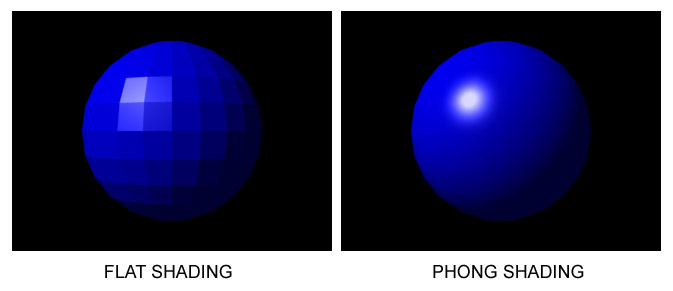
\includegraphics[width=\textwidth]{time_vs_quality}
    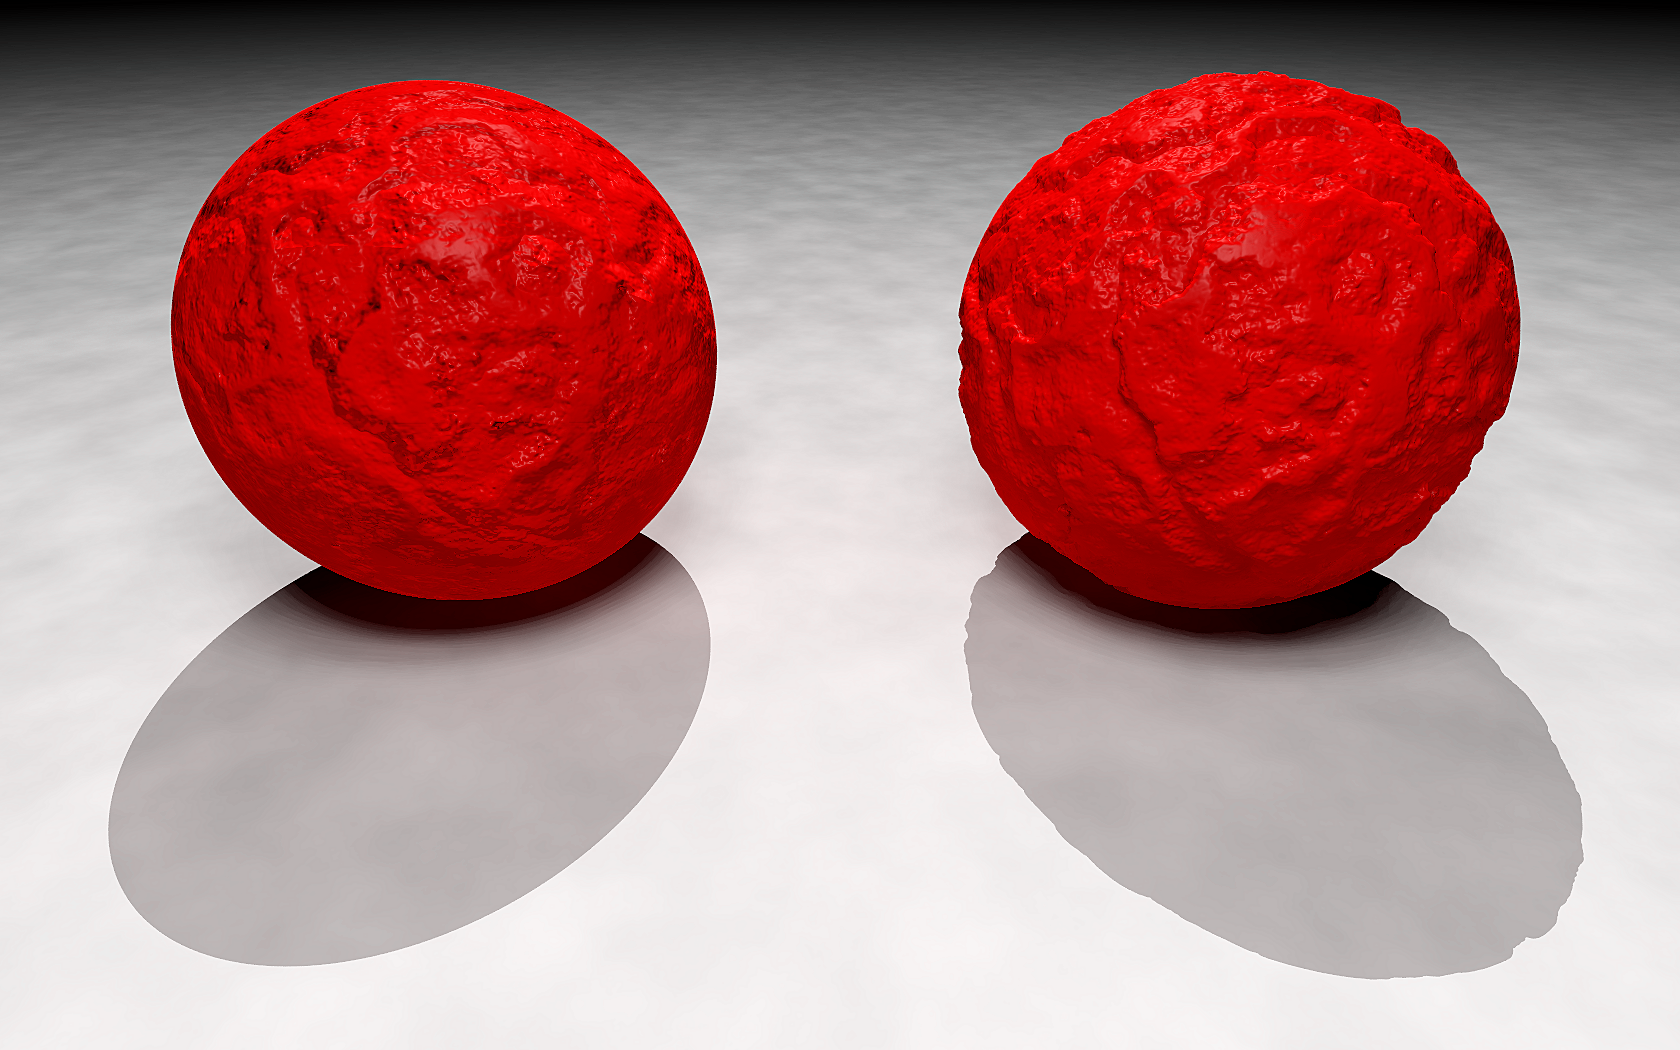
\includegraphics[width=\textwidth]{bumpmaps}
    \caption{Interpolation af flade-normaler kan få kantede figure til at få mere naturligt udseende.}
    \label{fig:tid_versus_kvalitet}
    % Demo der viser det samme http://math.hws.edu/graphicsbook/demos/c4/smooth-vs-flat.html
\end{figure}
\subparagraph{Rasterisering}
Den mest almindelige metode til at rendere miljøer med høj aktiv bruger interaktion er rasterisering. Rasterisering er også betegnelsen for at omdanne vector objekter til punkmatricer eller pixel-billeder (Se figur \ref{fig:pixelering}) Metoden virker ved at andvende linear transformationer på vektor objekter for at finde deres position på skærmen og derefter udfylde 2D polygonerne med farve, evt. baseret på forskællige lyskilder. Der kan dog simplificeres ved kun at andvende en ambient lys konstant. Rasterisering er også effektiv fordi grafikprocessore i computere er udviklet specifikt til at udføre matrix transformationer på store punktmængder.
\begin{figure}[H]
    \centering
    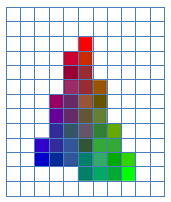
\includegraphics{rastarization_aprox}
    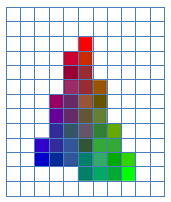
\includegraphics{rastarization_aprox}
    \caption{Pixelering der fremkommer når vektor objekter rastariseres.}
    \label{fig:pixelering}
\end{figure}
\subparagraph{Ray tracing}
% Kilder
% https://www.cs.unc.edu/~rademach/xroads-RT/RTarticle.html
% 
Raytracing er en metode som med relative simple regler, forsøger at andvende en fysisk model af lys, hvor fotoner spredes fra en lyskilde og rammer forskællige objekter indtil nogle få rammer øjet eller kamerarets optik. Raytracing simplificere ved at reducere problemet til kun at simulere de stråler der rammer vores øje. Dette gøres ved såkaldt \texit{backward ray tracing} hvorved man følger en stråle fra øjet, igennem computerskærmen og ind i vektormodellen hvor man tjekker for kollisioner mellem strålen og objekter. Ved kollision med reflektiktive objekter som metaliske overflader og gennemsigtige objekter som glas, vil strålen nu dele sig og følge f.eks gennem glasset men også følge en reflektiv vinkel for at udregne farven som den gennemsigtige/reflektive overflade har. For hver kollision følger man også en stråle mod alle lyskilder for at teste om der er objekter i vejen, således at kollisionspunktet ligger i skygge, da dette tages i betragtning som farven udregnes. Ved kollision med et mat objekt eller efter en forudbestemt antal reflektioner/refraktioner stopper udregningen og propagere tilbage igen.
\subparagraph{Radiosity}
% Kilder
% http://web.cs.wpi.edu/~matt/courses/cs563/talks/radiosity.html 
% http://www.cs.bath.ac.uk/~pjw/NOTES/75-ACG/ch5-radiosity.pdf
Hvor Rasterisering og raytracing udregner en pixels farve baseret på hvad man kan se igennem en skærmflade, så er radiosity en metode som er uafhængig af hvor kameraret er placeret og er af samme grund en af de mest tidskrævende metoder. (Måske er det muligt at precomputere modellen og så sende den til brugeren som kan interaktere med modellen via kameraret). Radiosity er baseret på en fysisk forståelse af lys interaktion med flader og fungere ved at alle flader absorbere en del af lyset der rammer dem og reflektere(radiates) resten som så går videre til at gentage processen for andre flader i scenen. Ved radiosity er lyskilder selv geometriske flader, hvilket gør det nemt at beskrive elementer som lamper og el-pærer. Karakteristisk for denne metode er såkaldt \textit{color bleeding}, hvor farver fra forskællige objekter smitter af på hindanden.
\begin{figure}[H]
    \centering
    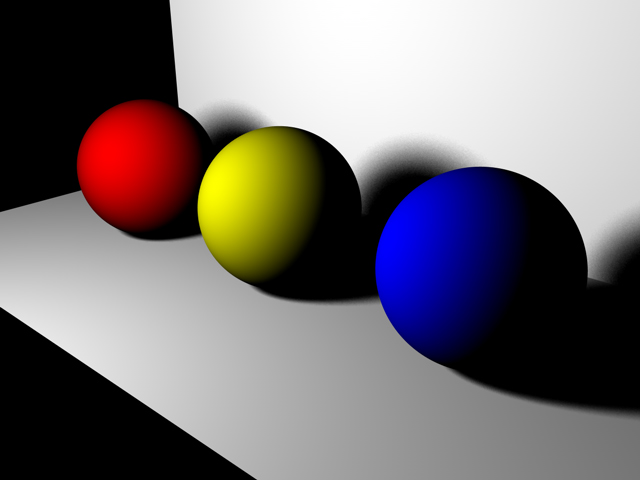
\includegraphics[width=6cm]{without_radiosity}
    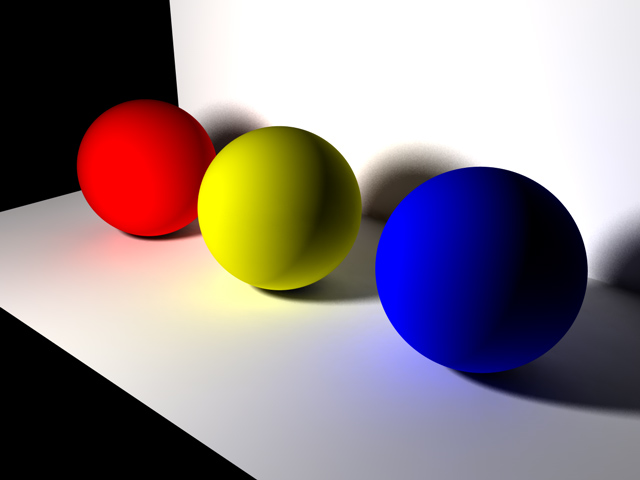
\includegraphics[width=6cm]{with_radiosity}
    \caption{\texit{Color bleeding} kan ses i billedet til højre.}
    \label{fig:colorbleeding}
\end{figure}

\clearpage


\section{Problemformulering}

Ud fra problemanalysen er vi blevet opmærksomme på følgende problem indenfor problemfeltet:
Det er et problem at kunden i en købssituation på e-butikker ikke kan visualisere, hvordan lys udbreder sig fra en lampe. Dette kan føre til fejlkøb af lamper, som påvirker både forbrugeren og e-butikken. For brugeren kan dette betyde irritation og i værste tilfælde kan det have sundhedsmæssige konsekvenser. For lampebutikker kan fejlkøb medføre utilfredse kunder og dårlig omtale. 

Dette fører os til det overordnede spørgsmål som vi ønsker besvaret i dette projekt:

\textit{Hvordan kan vi lave et værktøj til e-butikker, som vha.\ raytracing, visualiserer belysningen fra indendørslamper for kunderne?}

Herunder er der en række underspørgsmål, som ønskes besvaret:

\begin{enumerate}

\item \textit{Hvordan kan lampen visualiseres fra flere vinkler?}
\item \textit{Hvordan udbredes lyset fra en given lampe?}

\end{enumerate}


\renewcommand\refname{Bibliografi}
\begin{thebibliography}{99}

\section{Referencer}

\begin{thebibliography}{99}


\bibitem{kvalitativ_metode}
  Forklaring af kvalitativ metode,
  Den Store Danske.
  Set 25-11-2015.
  \url{http://www.denstoredanske.dk/Samfund,_jura_og_politik/Sociologi/Sociologisk_metodologi/kvalitative_metoder}

\bibitem{nummermetoden}
  Beskrivelse af nummermetoden, set 17-12-2015,
  \url{http://iva.ku.dk/refererkorrekt/tekshenvisninger/#Nummermetoden}

\bibitem{human_factors}
  Human Factors in Lighting, third edition,
  Peter R. Boyce, 2014.
  Sider 532-536.
  ISBN: 9781439874882.

\bibitem{ergonomi_arbejdsplads}
  Konsekvenser ved dårlig belysning på arbejdsplads mm.,
  ebscohost.
  Set 2-12-2015
  \url{http://web.b.ebscohost.com/ehost/detail/detail?sid=2898a5ec-e3ec-4bf2-b3b7-f4eb754cd767%40sessionmgr115&vid=0&hid=101&bdata=JnNpdGU9ZWhvc3QtbGl2ZQ%3d%3d#anchor=toc&db=buh&AN=7531667}

\bibitem{OSHA}
  Occupational Safety \& Health Administration,
  Set 16-12-2015.
  \url{https://www.osha.gov/}
  
\bibitem{CVS}
  Computer vision syndrom,
  gmj.
  Set 2-12-2015.
  \url{http://gmj.sljol.info/article/10.4038/gmj.v11i1.1115/galley/1023/download/}
  
\bibitem{ddo_visualisering}
  Definition af visualisering,
  Den danske ordbog.
  Set 27-10-2015.
  \url{http://ordnet.dk/ddo/ordbog?query=visualisere}
  
\bibitem{def_lys}
  Definition af lys,
  Videnskab dk.
  set 27-10-2015.
  \url{http://videnskab.dk/sporg-videnskaben/hvad-er-lys}
  
\bibitem{britannica_lys}
  Definition af lys,
  Britannica.
  Set 27-10-2015.
  \url{http://global.britannica.com/science/light}

\bibitem{integral_led}
  Om integral-led,
  integral-led.com.
  Set 2-11-2015.
  \url{http://www.integral-led.com/about-integral-led}
  
\bibitem{varm_kold}
  Definition af varm og kold lys,
  integral-LED.
  Set 27-10-2015.
  \url{http://www.integral-led.com/education/warm-white-or-cool-white}

\bibitem{american_heritage}
  American Heritage,
  The free dictionary.
  set 27-10-2015
  \url{http://www.thefreedictionary.com/lamp}

\bibitem{fysisk_kontra_online}
  The State of Retail 2015,
  Timetrade
  Sarah Wallace.
  Rapport udgivet i 2015.
  Side 22, figur 14.
  Copyright © 2015 by TimeTrade Systems, Inc.
  Set 3-11-2015.
  \url{http://www.timetrade.com/system/files/surveys/State_of_Retail_Report_Final_June15.pdf}

\bibitem{fortrydelsesret}
  Fortrydelse og returret,
  forbrug.dk.
  Set 28-10-2015.
  \url{http://www.forbrug.dk/Raad-og-rettigheder/Forbrugerleksikon/Fortrydelsesret}

\bibitem{ikea_returret}
  Ikeas returret,
  Ikea.
  Set 27-10-2015.
  \url{http://www.ikea.com/ms/da_DK/kundeservice/kundeservice_sporgsmaal_svar_kontakt_os.html?ICID=DKFOO_KONTAKT_230315}
  
\bibitem{ddo_ehandel}
  Definition af e-handel,
  Den Danske Ordbog.
  Set 26-10-2015.
  \url{http://ordnet.dk/ddo/ordbog?query=ehandel}

\bibitem{ddo_ebutik}
  Definition af e-butik,
  Den Danske Ordbog.
  Set 26-10-2015. 
  \url{http://ordnet.dk/ddo/ordbog?query=ebutik}

\bibitem{retsinformationen}
  Lov om forbrugeraftaler,
  Retsinformationen.
  Set 26-10-2015.
  \url{https://www.retsinformation.dk/forms/r0710.aspx?id=160666}

\bibitem{computergrafik_introduktion}
  A Short Introduction to Computer Graphics,
  Frédo Durand - MIT Laboratory for Computer Science.
  CSAIL.
  Set 5-11-2015.
  \url{http://people.csail.mit.edu/fredo/Depiction/1_Introduction/reviewGraphics.pdf}
  
\bibitem{Cylindo}
  Visual content and software as a service,
  Cylindo.
  Set 9-11-2015.
  \url{http://www.cylindo.com/}
  
\bibitem{rastarization} 
  Real-Time Massive Model Rendering, first edition, Sung-Eui Yoon, 2008. Side 31. ISBN: 9781598297928.

\bibitem{raytracing_for_begyndere}
  Ray Tracing: Graphics for the Masses, 
  Paul Rademacher of Department for Computer Science at the University of North Carolina at Chapel Hill.
  Department of Computer Science, University of North Carolina at Chapel Hill.
  Set 5-11-2015.
  \url{https://www.cs.unc.edu/~rademach/xroads-RT/RTarticle.html}

\bibitem{perspective_projection}
  Essential mathematics for games and interactive applications : a programmer's guide, second edition, James Van Verth \& Lars M   Bishop, 2008. Sider 212-236. ISBN: 9780080878614.
  
\bibitem{phong_paper}
  Illumination for computer generated pictures, Volume 18 Issue 6, Bui Tuong Phong \& Robert Ashenhurst, 1975. Sider 311-317. ISSN: 0001-0782.

\bibitem{stanford_phong}
  Raytracing, 
  CS148 AS3, Stanford University. 
  Set 01-12-2015.
  \url{http://graphics.stanford.edu/courses/cs148-10-summer/as3/instructions/as3.pdf}

\bibitem{tanner_helland}
  How to Convert Temperature (K) to RGB: Algorithm and   Sample Code,
  Tanner Helland.
  Set 04-12-2015.
  \url{http://www.tannerhelland.com/4435/convert-temperature-rgb-algorithm-code/}
  
\bibitem{charity_values}
  Blackbody color datafile, 
  Mitchell Charity. S
  et 04-12-2015.
  \url{http://www.vendian.org/mncharity/dir3/blackbody/UnstableURLs/bbr_color.htmle/}
  
\bibitem{tanner_helland_chart}
  Raw temperature vs RGB chart,
  Tanner Helland. 
  Set 09-12-2015.
  \url{http://www.tannerhelland.com/4435/convert-temperature-rgb-algorithm-code/raw_temperature_vs_rgb_chart/}

\bibitem{farvetemp}
  Beskrivelse af farvetemperatur, 
  Den Store Danske. 
  Set 13-12-2015.
  \url{http://www.denstoredanske.dk/It,_teknik_og_naturvidenskab/Elektricitet/Belysning/farvetemperatur}
  
\bibitem{solidworks}
  Liste af solidworks produkter, 
  solidworks. 
  Set 13-12-2015.
  \url{http://www.solidworks.com/sw/3d-cad-design-software.htm}

\bibitem{augmented_reality}
  Beskrivelse af augmented reality,
  Augmented Reality.
  Soha Maad
  Chapter 1, section 4
  ISBN 978-953-7619-69-5

\bibitem{artemides}
  Artemides Augmented Reality App, 
  Artemide.
  Set 14-12-2015.
  \url{http://www.artemide.com/blog/portfolio/the-new-version-of-artemide-augmented-reality-is-now-available/}

\bibitem{raytracingvsrastarizatioin}
  Fordele ved raytracing frem for rasterisering, set 16-12-2015,
  \url{http://www.tomshardware.com/reviews/ray-tracing-rasterization,2351-3.html}

\bibitem{softshadow}
  Beskrivelse af bløde skygger i raytracing, set 16-12-2015,
  \url{https://graphics.ethz.ch/teaching/former/seminar/handouts/Lang_SoftShadowVolumes.pdf}

\bibitem{rotationsmatricer}
  Weisstein, Eric W. "Rotation Matrix." From MathWorld--A Wolfram Web Resource, set 17-12-2015,
  \url{http://mathworld.wolfram.com/RotationMatrix.html}

%\bibitem{forbrugerportalen}
%  Definition af forbruger,
%  Forbrugerportalen
%  set 27-10-2015
  
%  \url{http://www.forbrugerportalen.dk/sider/artikel.asp?ID=13}


% \bibitem{prototyper_pdf}
%  Anvendelse af prototyper,
%  Teknologisk.dk
% set 27-10-2015
  
% \url{www.teknologisk.dk/_root/media/52285_Prototyping.pdf}

% \bibitem{fysiske_butikker}
% Forbrugere vil betale mere for varer i butikker,
% caltech.edu
% set 27-10-2015
  
% \url{http://www.caltech.edu/news/consumers-will-pay-more-goods-they-can-touch-caltech-researchers-say-1650}


% \bibitem{SolidWorks} 
%  3D CAD Software brugt af designere i IKEA,
%  set 17-11-2015
%  \url{http://www.3ds.com/products-services/solidworks/},
  
\end{thebibliography}
\clearpage

\end{thebibliography}
\end{document}
